%%%%%%%%%---Packages and document settings---%%%%%%%%%
\documentclass[twoside,twocolumn]{article}

  \usepackage{blindtext}      % Package to generate dummy text throughout this template 
  
  \usepackage[sc]{mathpazo}   % Use the Palatino font
  \linespread{1.05}           % Line spacing - Palatino needs more space between lines
  \usepackage[T1]{fontenc}    % Use 8-bit encoding that has 256 glyphs
  \usepackage{microtype}      % Slightly tweak font spacing for aesthetics
  
  \usepackage[spanish,es-tabla]{babel} % Language hyphenation and typographical rules
  \usepackage[utf8]{inputenc} % para poder utilizar acentos sin que te jodan
  
  \usepackage[hmarginratio=1:1,top=32mm,columnsep=20pt]{geometry}     % Document margins
  \usepackage[hang, small,labelfont=bf,up,textfont=it,up]{caption}    % Custom captions under/above floats in tables or figures
  \usepackage{booktabs}       % Horizontal rules in tables
  
  \usepackage{lettrine}       % The lettrine is the first enlarged letter at the beginning of the text
  
  \usepackage{enumitem}       % Customized lists
  \setlist[itemize]{noitemsep}  % Make itemize lists more compact
  
  \usepackage{mathtools}
  \DeclarePairedDelimiter\bra{\langle}{\rvert}        % Para notación de Dirac
  \DeclarePairedDelimiter\ket{\lvert}{\rangle}
  \DeclarePairedDelimiterX\braket[2]{\langle}{\rangle}{#1 \delimsize\vert #2}

  \usepackage{abstract}       % Allows abstract customization
  \renewcommand{\abstractnamefont}{\normalfont\bfseries}      % Set the "Abstract" text to bold
  \renewcommand{\abstracttextfont}{\normalfont\small\itshape} % Set the abstract itself to small italic text
  
  \usepackage{titlesec}                                   % Allows customization of titles
  \renewcommand\thesection{\Roman{section}}               % Roman numerals for the sections
  \renewcommand\thesubsection{\Roman{section}.\arabic{subsection}}         % roman numerals for subsections
  \renewcommand\thesubsubsection{\Roman{section}.\arabic{subsection}.\arabic{subsubsection}}   % roman numerals for subsections
  \titleformat{\section}[block]{\Large\scshape\centering}{\thesection.}{1em}{}    % Change the look of the section titles
  \titleformat{\subsection}[block]{\large}{\thesubsection.}{1em}{}                % Change the look of the section titles
  \titleformat{\subsubsection}[block]{\it}{\quad\footnotesize\thesubsubsection.}{0.5em}{}                % Change the look of the section titles
  %\titleformat{\paragraph}[block]{\it}{\quad\footnotesize:}{0.1em}{}                % Change the look of the section titles

  \usepackage{fancyhdr}     % Headers and footers
  \pagestyle{fancy}         % All pages have headers and footers
  \fancyhead{}              % Blank out the default header
  %\fancyfoot{}              % Blank out the default footer
  \fancyhead[C]{Detección de partículas con CMOS $\bullet$ Mayo 2018 $\bullet$ D. F. Balmaceda}   % Custom header text
  %\fancyfoot[RO,LE]{\thepage} % Custom footer text
  
  \usepackage{titling}      % Customizing the title section
  
  \usepackage{hyperref}     % For hyperlinks in the PDF
  \usepackage{graphics}     % standard graphics specifications
  \usepackage[demo]{graphicx}     % alternative graphics specifications
  \usepackage{subcaption}
  \usepackage{longtable}    % helps with long table options
  \usepackage{svg}          % para gráficos .svg
  \usepackage[binary-units=true]{siunitx}      % para las unidades
  \usepackage{datetime}

%%%%%%%%%---Title, authors, date & abstract---%%%%%%%%%
\title{Detección y análisis de interacciones de partículas con sensores APS-CMOS mediante la implementación de una librería en C++}
  \author{%
    \textsc{Darío Federico Balmaceda} \\[1ex]     %  Your name
    \normalsize Laboratorio Detección de Partículas y Radiación. Centro Atómico Bariloche \\        %  Your institution
    \normalsize \href{mailto:leschatten@gmail.com}{\texttt{leschatten@gmail.com}}                   %  Your email address
  }
  \date{\today}
  \renewcommand{\maketitlehookd}{
    \begin{abstract}\noindent
      Los sensores CMOS constituyen una alternativa de bajo precio para la detección de eventos de partícuals.
      En este trabajo se implementó una librería para utilizar el sensor OmniVision OV5647
      de la cámara Raspicam V1.3, con una Raspberry Pi.
      \\ \noindent
      Utilizando esta librería se observó la presencia de los picos de emisión de rayos X
      $K_{\alpha}$ y $K_{\beta}$ del Cu y los picos $K_{\alpha}$ del Fe y del Ca.
      La determinación de estos picos permitió hacer la correcta calibración de carga depositada en
      función del valor de los píxeles.
      Además se utilizó la librería para la detección de interacciones del sensor con partículas
      producidas por rayos cósmicos.
      %TODO: ABSTRACT
    \end{abstract}
  }

  \setlength{\droptitle}{-4\baselineskip}                 % Move the title up
  \pretitle{\begin{center}\Large\bfseries}                 % Article title formatting
  \posttitle{\end{center}}                                % Article title closing formatting

%
  %%%%%%%%%%%%%%%%%%%%%%%%%%%%%%%%%%%%%%%%%%
  %%%%                                 %%%%%
  %%%%  And now, begin the document... %%%%%
  %%%%                                 %%%%%
  %%%%%%%%%%%%%%%%%%%%%%%%%%%%%%%%%%%%%%%%%%
\begin{document}
  
  \maketitle              % Print the title
  
  %%%%%%%%%%%%%%%%%%%%%%%%%%%%%%%%%%%%%%%%%%%%%%%%%%%
  \section{Introducción}\label{sec:intro}
    \lettrine[nindent=0em,lines=3]{L}os sensores de imágenes CMOS son ampliamente utilizados en los dispositivos electrónicos comerciales
    debido a su bajo costo de producción. Estos están presentes en celulares, consolas de videojuegos, cámaras de acción,
    sistemas de seguridad y un sinfín de aplicaciones más.
    En el ámbito científico, estos sensores están comenzando a tener relevancia \cite{PerezCMOS},
    ya que permiten realizar estudios de dosimetría, calcular actividad de muestras radioactivas y control de reactores nucleares
    a un coste muy inferior que al de los CCDs utilizados para determinar la carga depositada en las interacciones sensor-partícula.
    Como en experimentos como DAMIC (búsqueda de materia oscura)\cite{DAMIC}
    o CONNIE (medición de neutrinos)\cite{CONNIE}.

    En base a esto se propone implementar una librería con filosofía de programación orientada a objetos
    capaz de hacer uso de estos sensores CMOS para la detección de interacciones de partículas con el sensor,
    y poder estimar parámetros como el número de eventos en una imagen (fotograma) y la carga de estos eventos.

    \subsection{Sensores CMOS-APS}\label{sec:intro:CMOS_sensor}
      Un sensor de píxeles activos (APS por sus siglas en inglés) es un sensor que detecta la radiación utilizando tecnología CMOS.
      La tecnología CMOS hace referencia a un conjunto de familias lógicas basadas en semiconductores complementarios de óxido metálico,
      estos utilizan transistores de tipo pMOS y de tipo nMOS, de esta forma el único consumo en reposo se debe a las corrientes parasitarias.

      Estos sensores consisten en un arreglo matricial de fotodiodos,
      que producen una corriente de electrones que varía en función de la intensidad de luz recibida,
      basándose en el efecto fotoelectrico para la generación de pares electrón-hueco.
      Por cada fotodiodo se incorpora un amplificador. Según el diseño, se incorpora
      un conversor analógico digital (ADC) para la lectura de los datos, a cada píxel o por columnas.

    \subsubsection*{\hspace{5mm}Filtro de Bayer}\label{sec:intro:bayer}
      Los sensores CMOS destinados para fotografías a color poseen un filtro de Bayer, 
      el mismo consiste en un arreglo de filtros rojos, verdes y azules dispuestos como se muestra en la Fig.~\ref{fig:bayer}.
      De esta forma, cada píxel posee la información de un único rango de longitudes de onda, 
      esto permite una composición de la imagen en 3 colores diferentes, de manera análoga al ojo humano.
      Para formar la imagen final en una fotografía, se utiliza un algoritmo de des-Bayerización.\cite{picamera}

      \begin{figure}[h]
        \centering
        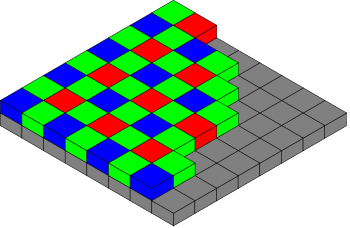
\includegraphics[width=0.35\textwidth]{figures/Bayer_pattern.png}
        \caption{Filtro de Bayer típico de un sensor CMOS-APS. Cada 4 píxeles hay 2 con filtro verde, 1 con rojo y el último con es azul.
          El color verde es utilizado dos veces debido a la sensibilidad al verde del ojo humano.}
        \label{fig:bayer}
      \end{figure}

      Si bien este filtro resulta invisible a los rayos X,
      y no es relevante en el caso de un snsor CMOS para detectar partículas;
      el distinguir fotografías por sus colores permitió caracterizar
      de los distintos parámetros a la hora del tomar una fotografía,
      tal como se describe en el apéndice~\ref{sec:ap_alternatives}.

    \subsection{Detección de partículas con el sensor CMOS}\label{sec:intro:detection}   

      Una partícula de energía que deposite una energía $E$ en el sensor,
      es capaz de generar $E / a$ pares de electrón-hueco,
      siendo $a$ la energía promedio para generar un par electrón-hueco en el material
      \footnote{\SI{3.7}{\eV} en el caso del silicio\cite{groom2004temperature}}.
      El valor máximo de electrones hasta llegar a saturación es conocido como \emph{Full Well Capacity}.

      Si la densidad de eventos en una imagen es baja\footnote{En relación con el tamaño de los eventos},
      es posible identificar eventos a partir de los pixeles de una vecindad,
      debido a que se desprecia la probabilidad de encontrar un píxel que haya acumulado carga de dos eventos distintos.
      En caso de haber una densidad de eventos mayor, pueden utilizarse otros métodos, como técnicas basadas en
      algoritmos de aprendizaje profundo (\emph{deep learning}) e inteligencia artificial. \cite{ROE2005577} 
      
    \subsection{Fluorescencia de rayos X}\label{sec:intro:peaks}

      La emisión de rayos X característicos corresponde a la ionización de un átomo en la que un
      electrón de las primeras capas es excitado a un estado no ligado.
      En este caso un electrón de una capa superior ocupa la vacante dejada por el electrón.
      Durante este proceso, dado que la energía se conserva, se emite un fotón
      cuya energía es igual a la diferencia entre los niveles de la transisición.

      Los picos $K_\alpha$ y $K_\beta$ corresponden a las transiciones de un electrón de un estado
      $\ket{2p}$ al estado $\ket{1s}$ y a la transición $\ket{3p}$ a $\ket{1s}$, respectivamente.
      
      En el caso particular del Cu, Fe y Ca, 3 elementos que usaremos a continuación,
      los valores de energía de los fotones emitidos se pueden encuentrar
      en la Tabla~\ref{tab:xraypeaks}.

      \begin{table}[h]
        \centering
        \begin{tabular}{|rl|ll|l|} \hline
        \textbf{Z}  & \textbf{\small{Elem.}} & $K_{\alpha_1}$ & $K_{\alpha_2}$ & $K_\beta$ \\ \hline
        \textbf{20} & \textbf{Ca}       & 3692         & 3688         & 4012        \\
        \textbf{26} & \textbf{Fe}       & 6404         & 6391         & 7058        \\
        \textbf{29} & \textbf{Cu}       & 8048         & 8028         & 8905       \\ \hline
        \end{tabular}
        \caption{Valores de energía, en eV, de los fotones emitidos para los picos de emisión 
          $K_{\alpha}$ y $K_{\beta}$ del Ca, Fe y del Cu.\cite{xraybooklet}.}
        \label{tab:xraypeaks}
        \end{table}

    \subsection{Rayos cósmicos}\label{sec:intro:cosmic_ray}
      Los rayos cósmicos son partículas que llegan desde el espacio y bombardean constantemente la Tierra desde todas direcciones.
      La mayoría de estas partículas son protones o núcleos de átomos.
      Al interactuar con la atmósfera terrestre, los rayos cósmicos de alta energía (mayor a \SI{}{10^{20}\eV})
      son capaces de producir hadrones cargados, neutrones, fotones (rayos $\gamma$),
      muones (de 1 a 5 \si{\giga \eV}), electrones y positrones (de 1 a 20 \si{\mega \eV}), \cite{GriederCRAE}
      cuyos efectos son medibles.
      %TODO: Poner algunos valorcitos
  

  %%%%%%%%%%%%%%%%%%%%%%%%%%%%%%%%%%%%%%%%%%%%%%%%%%%
  \section{Configuración experimental}\label{sec:conf_exp}

    \subsection{Sensor CMOS}\label{sec:conf_exp:CMOS}
      Se ha utilizado el sensor OmniVision OV5647 de la cámara Raspicam V1.3 cuyo precio ronda los 23 dólares.
      El sensor posee	$2592$x$1944$ píxeles, lo que le da una resolución total de $5$ MP.
      El tamaño de un píxel de \SI{1.4}{\micro\meter} x \SI{1.4}{\micro\meter}.
      La capacidad de carga máxima hasta llegar a saturación es de $4300$ electrones (\emph{Full Well Capacity}).
      El sensor posee un ADC de 10 bits por píxel.
      El tamaño total por imagen raw es de unos \SI{6.4}{\mega\byte}.

    \subsection{Raspberry}\label{sec:conf_exp:raspberry}
      Se utilizó una Raspberry Pi modelo B, con una memoria micro SD de \SI{16}{\giga\byte}, para la obtención de imágenes.
      Debido a la resolución de las imágenes, la profundidad de bits de la imagenes y del tamaño del sistema operativo \emph{Raspbian}, 
      la memoria disponible permitió almacenar del orden de 1000 fotografías en simultáneo.

    \subsection{Librería raspiraw}\label{sec:conf_exp:raspiraw}
      Para la adquisicón de datos se utilizó la librería {\it raspiraw}\cite{raspiraw} debido a la rapidez con la que se toman los datos.
      En el apéndice~\ref{sec:ap_alternatives} se muestran otras alternativas que son más lentas para la toma de datos,
      pero que pueden resultar más simples y sencillas de implementar.

      Los datos sin procesamiento (datos \emph{raw}) se almacenaron con extensión \emph{.raw}.
      El valor de carga acumulada por cada píxel se representa mediante un número de $10$~bits.
      En una misma fila, los píxeles son agrupados de a $4$, formando una estructura de $5$~bytes.
      En los primeros $4$~bytes se encuentran los bits más significativos de los 4 píxeles que conforman la estructura.
      El quinto byte contiene los últimos $2$~bits menos significativos de cada píxel.\cite{picamera}
      La manera en la que los bits están ordenados en un grupo se muestra en la Fig.~\ref{fig:arreglo}

      \begin{figure}[h]
        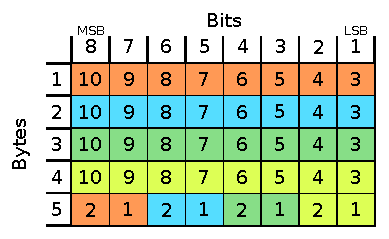
\includegraphics[width=0.47\textwidth]{figures/bayer_bytes.pdf}
        \caption[LoF entry]{Representación de un grupo 4 píxeles.

        Los $40$~bits de los $4$ píxeles están distribuídos como ilustra la figura.
        Colores distintos corresponden a píxeles distintos.

        En cada celda se encuentra un número que representa el bit de información de un píxel,
        siendo 1 el bit menos signficativo (LSB) y 10 el bit más signficativo (MSB).}
        \label{fig:arreglo}
      \end{figure}

      Estos datos consistían en $1952$ filas de 3264~bytes.
      Las últimas $8$ filas de datos no contienen información y no son utilizadas,
      ya que sólo existen debido a que $1952$ es menor múltiplo de $16$
      mayor a las $1944$ filas que posee el sensor (ver sección \ref{sec:conf_exp:CMOS}).
      De la misma forma, los último $24$~bits de cada fila no son utilizados y deben ser descartados.

      Esta librería permite cambiar varios parámetros de la toma de datos.
      En partícular, los parámetros que se modificaron son son:
      \paragraph{Tiempo de exposición:}
        Se define como el tiempo en el que sensor acumula carga.
        A mayor tiempo de exposición, mayor es la carga leída por el detector,
        cuando se encuentra expuesto a una fuente de luz.
        
        En lo que sigue, se utilizó un tiempo de exposición de \SI{500}{\milli\second}, a no ser que se aclare lo contrario.

      \paragraph{Cuadros por segundos:}
        También conocido como \emph{fps} por sus siglas en inglés.
        Se refiere a la frecuencia con la que se toman las imágenes y generalmente viene expresado en fotografías por segundo.
        
        En lo que sigue, se capturó a 2 cuadros por segundo, a no ser que se aclare lo contrario.

      %\paragraph{Ganancia}

    \subsection{Librería propia}\label{sec:conf_exp:library}
      Para el procesamiento de las imagenes de raspiraw se implementó una librería en C++. En esta librería las imágenes pasan
      a ser objetos representados por una matriz (arreglo modulado). Cada foto presenta un ancho, un largo y un conjunto de datos que
      corresponder al valor de cada pixel. En esta clase se definen los métodos (funciones) para encontrar eventos, basándose en
      pixeles adyacentes, para recortar imágenes, encontrar el valor medio, la mediana y hasta para encontrar
      la desviación estándar de los valores de los pixeles.

      A su vez, cada evento es representado por otra clase cuya identidad viene dado por una lista de pixeles (posición horizontal,
      posición vertical y valor). Para esta clase se definen métodos que permiten
      obtener la carga total de un evento, definida como la suma de los valores de los pixeles;
      para obtener el centro de masa del evento,
      definida como el promedio de los vectores posiciones de cada pixel,
      ponderado con el valor del pixel;
      para determinar el radio de un evento, definido como la raiz cuadrada de la varianza de las posiciones
      de los pixeles al centro de masa, también ponderado por el valor de cada pixel.

      El código fuente puede encontrarse en la plataforma GitHub mediante el siguiente enlace
      \href{https://github.com/DBFritz/ParticleDetections}{\texttt{github.com/DBFritz/ParticleDetection}}

    \subsection{Emisor de rayos X}\label{sec:conf_exp:x-rays}
      En la Fig.\ref{fig:photo_xray} se muestra la configuración experimental utulizada.
      La cámara de la Raspberry Pi se colocó en un recipiente de plástico opaco a la luz visible,
      para evitar detectar los fotones en ese rango de longitudes de onda.
      El equipo utilizado posee dos ventanas, se utilizó la menos coherente para facilitar el proceso
      de alineado del haz con la cámara. 
      
      El generador de rayos X utilizado corresponde al grupo de materiales del Centro Atómico Bariloche,
      el mismo utiliza la diferencia de energía entre los niveles del Cu para generar los rayos X.
      Por este motivo, la emisión de los rayos X no corresponde a un espectro uniforme, sino que presenta
      máximos locales en los valores que corresponden a diferencias de niveles energéticos.
      
      Para la medición de los picos de Fe y Ca se intercaló una lámina de Fe y una concha marina (rica en Ca).
      Debido a que los rayos X se generan en base al Cu, los picos de emisión también estarán presentes en
      el espectro de los demás elementos.

      \begin{figure}[h]
        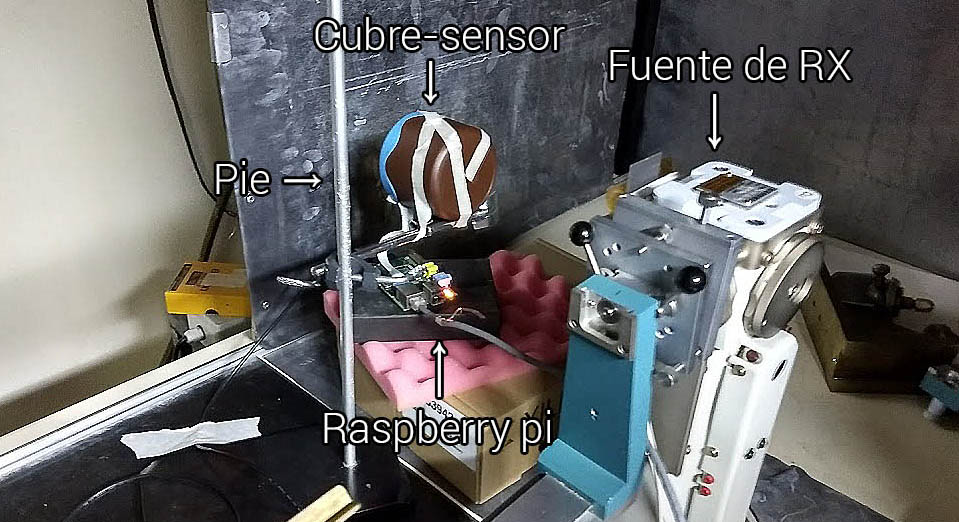
\includegraphics[width=0.47\textwidth]{figures/IMG_20180412_173110355_HDR}
        \caption{Configuración experimental utilizada para la detección de rayos X.
        El sensor se colocó dentro de un recipiente plástico para protogerla de la luz visible.
        El pie permitía alinear correctamente el haz de fotones con la cámara.
        }
        \label{fig:photo_xray}
      \end{figure}

    \subsection{Observación de rayos cósmicos.}\label{sec:conf_exp:cosmic_ray}
      Utilizando la librería propia desarrollada e en el marco de este proyecto (ver sección \ref{sec:conf_exp:library}),
      es posible idenficar eventos en paralelo con la toma de imágenes,
      por lo que se implementó un sistema que guarde solamente las imágenes que poseen pixeles que superen un umbral establecido.
      Permitiendo así medir durante días sin saturar la memoria, eliminando las fotos vacías de eventos.
      Debido al ruido de lectura, dicho umbral se ajustó en $75$ Unidades de ADC. %FIXME: BERTOU: sección 3.1!? 
      Como se verá en la sección \ref{sec:results:cosmic_ray}, con esta configuración fue posible detectar eventos,
      por lo que el umbral establecido resultó válido y suficiente.
      Se tomaron 2 imágenes por segundo, pero éstas eran procesadas a una velocidad
      del orden de 1 imagen cada 3 segundos, por lo que se espera que la frecuencia de eventos
      detectados debido a rayos cósmicos sea notablemente menor a la frecuencia de eventos conocida,
      que es del orden de \SI{100}{\meter^{-2}\second^{-1}}
      (para una sección de \SI{10}{\milli\meter^2}, casi 4 eventos por horas).
      %FIXME: Digo que frecuencia y la mido en Hz/area

  %%%%%%%%%%%%%%%%%%%%%%%%%%%%%%%%%%%%%%%%%%%%%%%%%%% 
  \section{Resultados y discusión}\label{sec:results}
    Se probó el correcto funcionamiento de la librería, descripta en la sección \ref{sec:conf_exp:library},
    en tres aplicaciones diferentes.
    En primer lugar se determinó el ruido de lectura de la cámara,
    otra de ellas consistió en observar los picos $K_{\alpha}$ y $K_{\beta}$ de diferentes elementos
    para calibrar la respuesta del sensor,
    y por último, en detectar rayos cósmicos.

    \subsection{Determinación del ruido de lectura}\label{sec:results:background}
      Se realizó un histograma de los valores de los pixeles de una única imagen,
      para verificar la distribución y la dispersión del ruido.
      Los resultados obtenidos se muestran en la Fig.~\ref{fig:histogram}.

      \begin{figure}[h]
        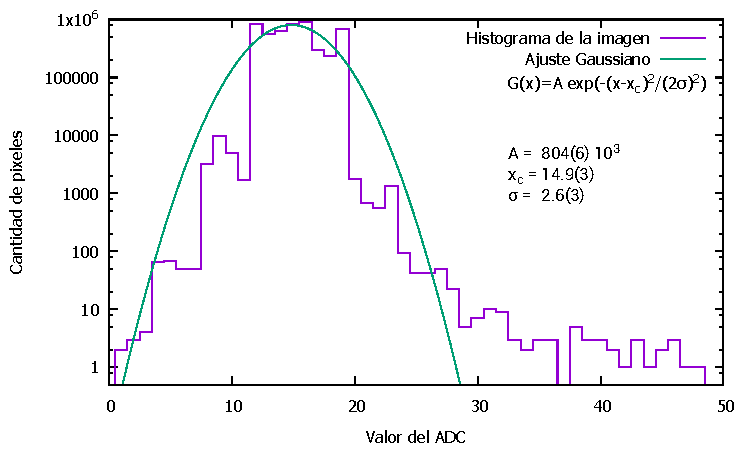
\includegraphics[width=0.45\textwidth]{figures/background_histo.pdf}
        \caption{Histograma de los valores de los pixeles con un ajuste gaussiano.
          El histograma se muestra en escala logarítmica.
          La gaussiana se encuentra centrada en $14.9(3)$ unidades de ADC,
          mientras que su dispersión es $2.6(3)$ unidades de ADC.}
        \label{fig:histogram}
      \end{figure}

      Se observa que el ruido está muy alejado de uin comportamiento de ruido blanco (gaussiano),
      indicando la presencia de un FPN (ruido de patrón fijo).
      
      Se tomaron 30 imágenes con tiempo de exposición de \SI{500}{\milli\second} a 2 cuadros por segundos (\emph{fps}).
      Se promediaron las 30 imágenes para obtener una estimación sobre el ruido de lectura con la configuración dada. 
      En la Fig.~\ref{fig:background} se muestra el promedio por píxel de las fotografías tomadas.

      \begin{figure}[h]
        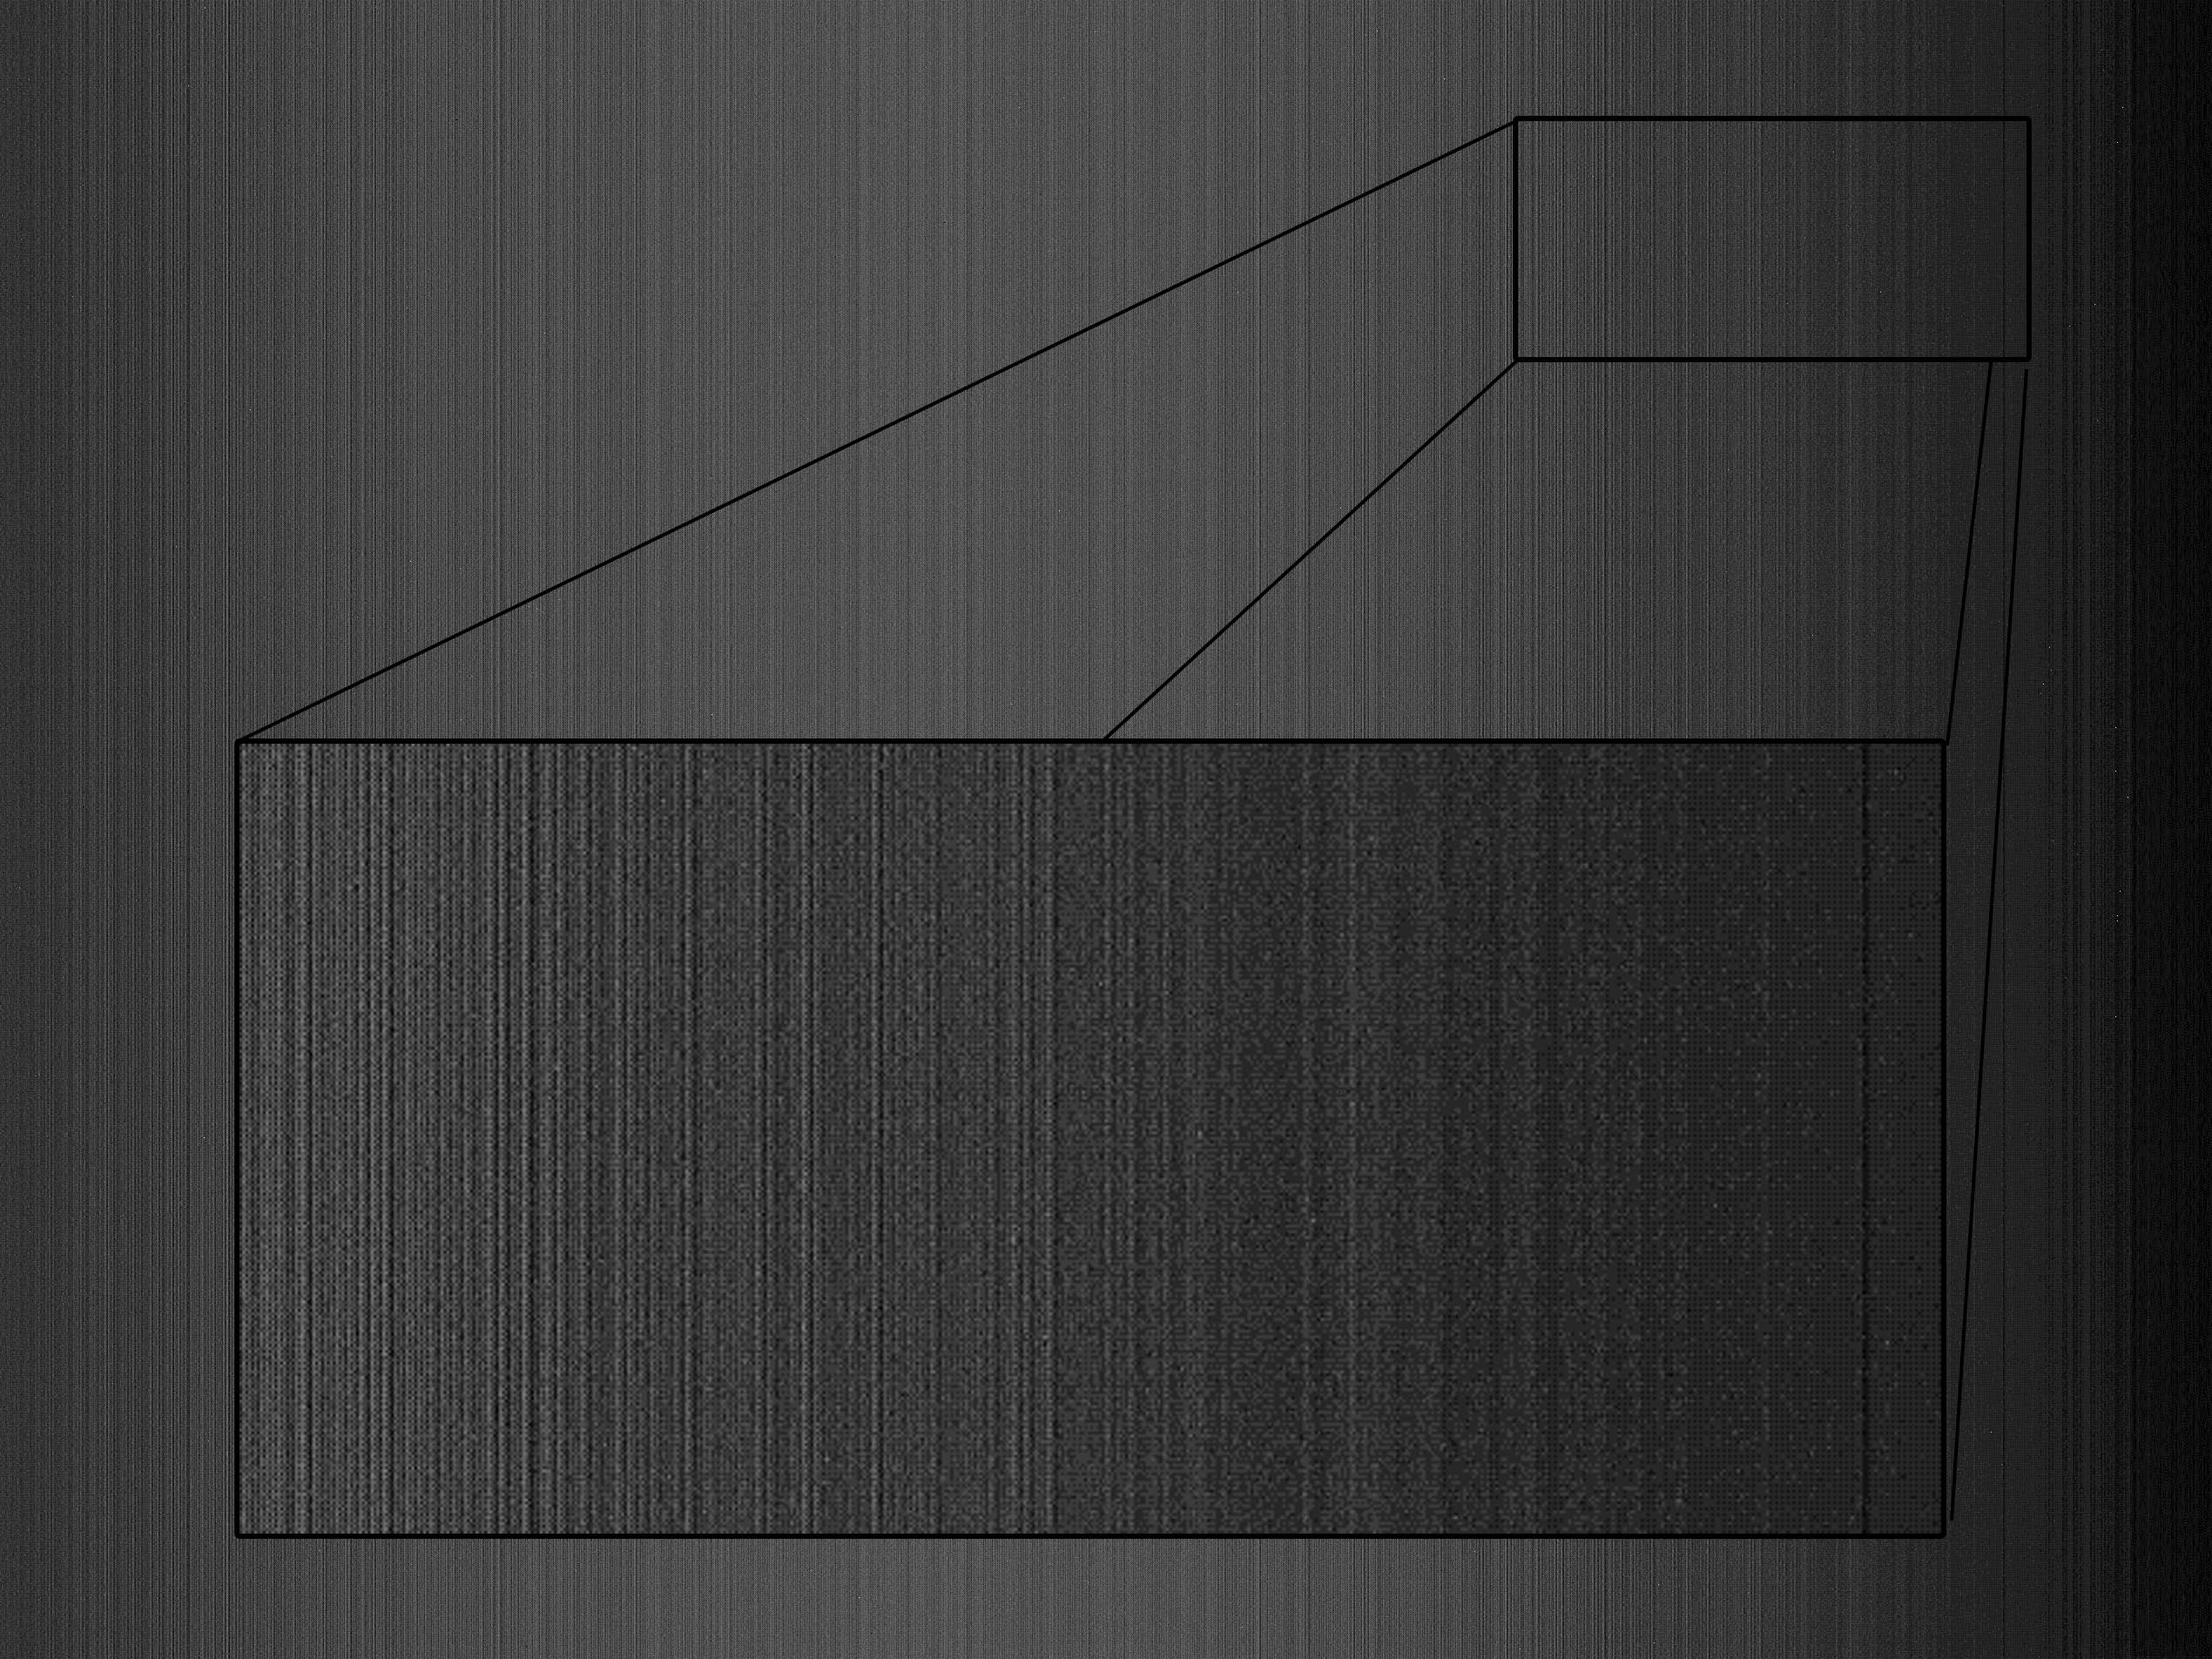
\includegraphics[width=0.47\textwidth]{figures/background.jpg}
        \caption{Promedio de las 30 imagenes del fondo. 
          Se observa una dependencia del valor promedio como función de la posición.
          Esta dependencia está fuertemente relacionada con la columna del píxel. }
        \label{fig:background}
      \end{figure}
    
      En base a la fuerte dependencia del valor medio de los pixeles como función de la columna,
      se implementó una función que permite sustraer, a cada columna, el valor medio por columna.
      Esta función será aplicada a cada procesamiento de datos de imágenes, salvo que se indique lo contrario.
      Se recalculó el histograma de la misma imagen que en la Fig.~\ref{fig:histogram}, con la respectiva sustracción
      de la mediana por columna. Dicho histograma se muestra en la Fig.~\ref{fig:histogram_subs}.

      \begin{figure}[h]
        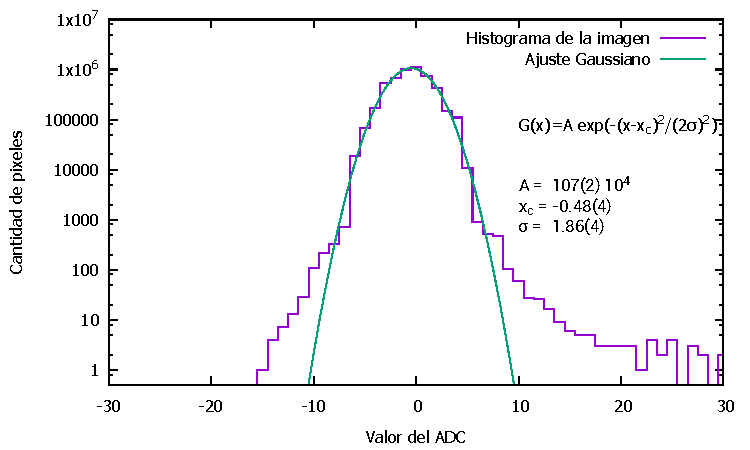
\includegraphics[width=0.47\textwidth]{figures/background_histo_subs.pdf}
        \caption{Histograma de los valores de los pixeles, después de corregir por columna, con un ajuste gaussiano.
        El histograma se encuentra en escala logarítmica.
        Los valores obtenidos del ajuste se muestran en el gráfico.}
        \label{fig:histogram_subs} %TODO: Ampliar el caption.
      \end{figure}

      En este caso se observa un comportamiento notablemente más gaussiano, con una dispersión es un $28\%$ menor.

    \subsection{Mediciones de picos $K_{\alpha}$ y $K_{\beta}$ y calibración de energía}\label{sec:results:peaks}
      Se analizó el espectro de Cu, Fe y Ca utilizando la librería propia, descripta en la sección \ref{sec:conf_exp:library}.
      Para esto, se realizó un histograma de las cargas de los eventos del orden de 300 imágenes.
      En estos espectros fue posible identificar los picos $K_{\alpha}$ y $K_{\beta}$ de Cu y los picos $K_{\alpha}$ del Fe y del Ca,
      tal como se muestra en la Fig.~\ref{fig:spectrum_x-ray}.

      \begin{figure}[h]
        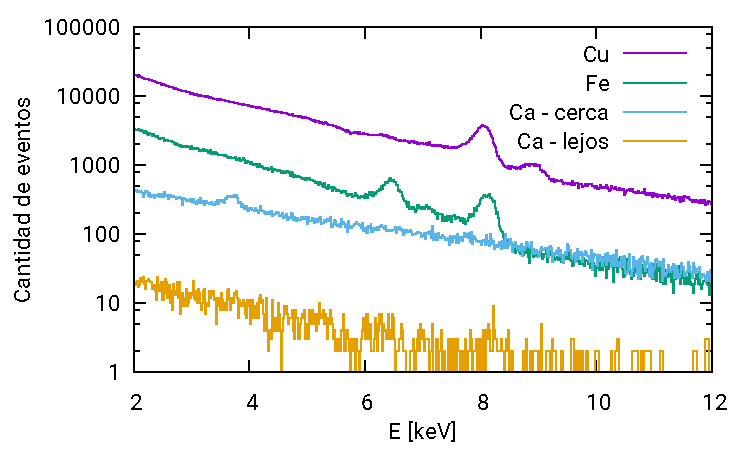
\includegraphics[width=0.47\textwidth]{figures/x-ray_spectrum.pdf}
        \caption{Espectro detectado por el sensor. \\
          El espectro del Cu corresponde al espectro de emisión de la fuente utilizada.
          Los demás espectros se obtuvieron colocando una placa de Fe y de Ca, respectivamente,
          entre la fuente y el sensor.
          En el gráfico ya se ha realizado la calibración entre energía y unidades de ADC mostrada en la Fig.\ref{fig:x-ray_calibration}}
        \label{fig:spectrum_x-ray}
      \end{figure}

      En el caso del espectro del Fe, puede observarse la presencia del pico $K_\alpha$ del Cu, debido a que la fuente es de Cu.
      De la misma forma, este pico puede verse en el caso del espectro del Ca cuando éste fue ubicado lejos del sensor.

      Conociendo la energía característica de cada uno de estos picos \cite{xraybooklet},
      y bajo la suposición que los electrones generados pierden todas su energía, % FIXME: Poner la consideración de que el fotón se frena
      se realizó una calibración del valor raw de un pixel como función de la carga (energía) depositada.
      Esta calibración se muestra en la Fig.~\ref{fig:x-ray_calibration}

      \begin{figure}[h]
        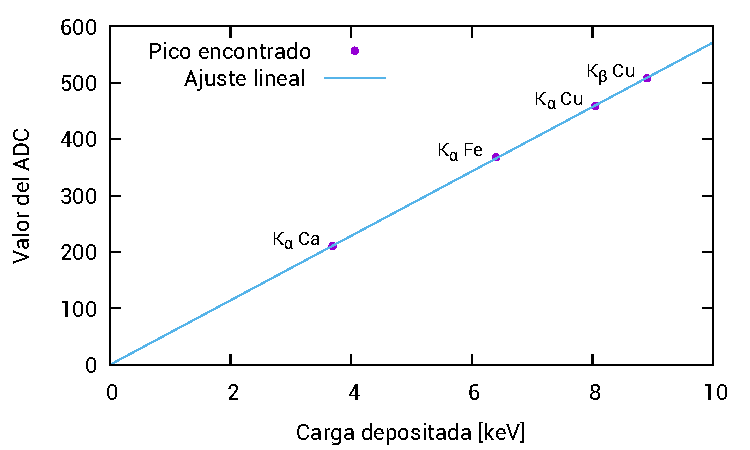
\includegraphics[width=0.47\textwidth]{figures/x-ray_calibration}
        \caption{Calibración del canal del sensor como función de la energía de
          los picos $K_{\alpha}$ y $K_{\beta}$ encontrados.
          En el mismo se puede apreciar que la relación es lineal,
          y la relación carga por unidad de ADC obtenida es de \SI{17.50(3)}{\eV}
        }
        \label{fig:x-ray_calibration}
      \end{figure}

    \subsection{Medición de Rayos Cósmicos}\label{sec:results:cosmic_ray}
      Utilizando la librería propia, se pudo encontrar $2$ %TODO: Poner el valor
      eventos en 2 días seguidos, con la cámara en oscuridad y sin la presencia de fuentes radioactivas cerca,
      por lo que se asocia estos eventos a los rayos cósmicos.
            %FIXME: No se puede asegurar que sean muones, sadly :'(
      En la Fig.~\ref{fig:cosmic_ray} se muestran ambos eventos detectados.

      \begin{figure}[h]
        \centering
        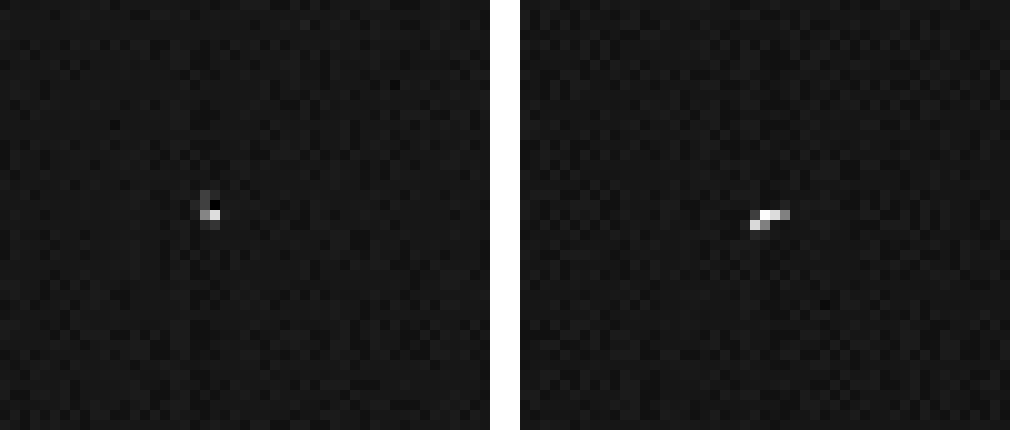
\includegraphics[width=0.47\textwidth]{figures/doble_evento.png} % TODO: Poner para que salga pixelada :(
        \caption{Recortes de las imágenes tomadas en la que se observaron un evento de rayos cósmicos.
        En este caso el color negro representa el 0 unidades de ADC, y el color blanco, 180 unidades de ADC (\SI{3150}{\eV}).
        }
        \label{fig:cosmic_ray}
      \end{figure}

      %TODO: Hacer la cuenta!!!

  %%%%%%%%%%%%%%%%%%%%%%%%%%%%%%%%%%%%%%%%%%%%%%%%%%%
  \section{Conclusiones}
    Se utilizaron sensores CMOS para la detección de eventos con partículas para una descripción cualitativa y esquemática.
    Se analizó la dependencia con los distintos parámetros de la cámara y en base a esto se decidió una configuración de trabajo.

    Gracias a esto se pudo caracterizar y calibrar el sensor para la configuración utilizada mediante la implementación de la librería
    en C++ con filosofía de Programación Orientada a Objetos.
    Utilizando esta librería se observó la presencia de eventos producidos por rayos cósmicos y
    se observaron los picos $K_{\alpha}$ y $K_{\beta}$ del Cu y los picos $K_{\alpha}$ del Fe y Ca.

    El alcance de esta librería es amplio. Uno de los posible usos es la detección de fuentes radioactivas, como el plomo,
    en el agua. Además podría utilizarse como un contador de contador de Geiger barato.

  %%%%%%%%%%%%%%%%%%%%%%%%%%%%%%%%%%%%%%%%%%%%%%%%%%% 
  \bibliographystyle{unsrt}
  \bibliography{bibliography}

  %%%%%%%%%%%%%%%%%%%%%%%%%%%%%%%%%%%%%%%%%%%%%%%%%%%
  \section*{Agradecimientos}
    Se agradece la colaboración de Xavier Bertou por la experiencia brindada y por
    acompañar el trabajo en forma constante.
    A Miguel Sofo por la disponibilidad y por la ayuda a la hora de hacer mediciones.
    % TODO: Agregar a alguien que Bertou me dijo pero me colgué
    % Era del grupo de José por proveernos de los rayos X
    Al equipo de Fabricio Alcalde por proveernos e informarnos sobre el equipo de rayos X.

  %%%%%%%%%%%%%%%%%%%%%%%%%%%%%%%%%%%%%%%%%%%%%%%%%%%
  \clearpage
  \appendix
  \section{Alternativas a Raspiraw}\label{sec:ap_alternatives}
  
  \subsection*{Raspistill y Raspivid}
    Ambos vienen por defectos instalados en el sistema operativo \emph{Raspbian}.
    Raspistill permite capturar fotografías en formato \emph{Joint Photographic Experts Group} (jpeg/jpg).
    Si bien las imágenes tomadas presentan un post-procesamiento, Rapistill es capaz de añadir a la imagen los datos sin procesar (\emph{raw}),

    Por el otro lado, raspivid permite grabar videos en formato \emph{H.264}.
    Este formato también presenta compresión de datos, al igual que \emph{.jpg},
    pero no existe parámetro que permita obtener las imágenes sin procesamiento.
    Por lo solamente debe ser utilizado de manera ilustrativa y cuantitativa, pero no cuantitativa.

    Para verificar el funcionamiento del sensor, se expuso la cámara ante una fuente de rayos alfa ($^{241}$Am),
    removiendo previamente el sistema óptico de lentes que poseía la cámara \emph{picamera}.
    Utilizando raspivid, se tomó 1 minuto de exposición a 30 cuadros por segundos, dando un total de 1800 imágenes.
    Por pixel, se tomó el máximo valor de todas las imágenes, generando la imagen que se muestra en la Fig.~\ref{fig:raspivid}

    \begin{figure}[h]
      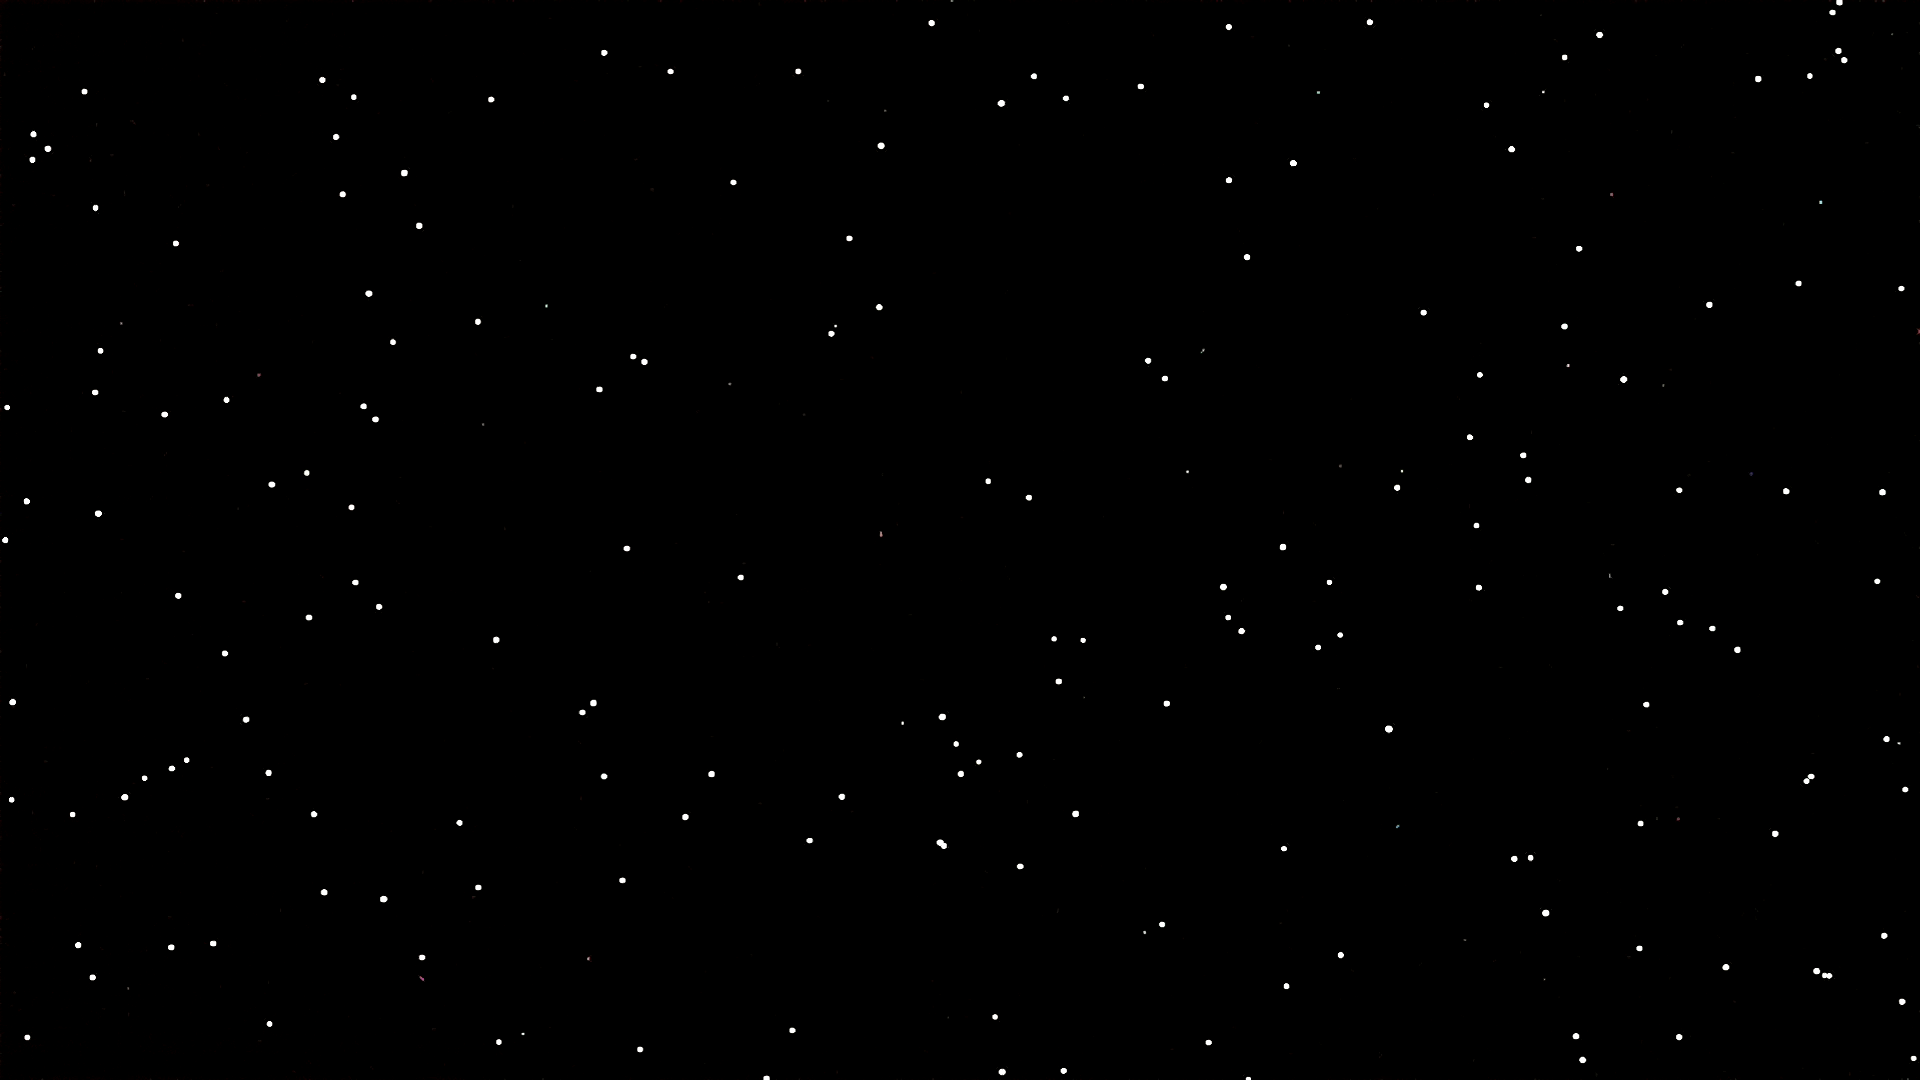
\includegraphics[width=0.47\textwidth]{figures/Alpha_1m.png}
      \caption{Imagen de los eventos con exposición de 1 minuto ante una fuente de $^{241}$Am,
      que emite radiación alfa de \SI{5.486}{\mega\eV}.
      Para la composición de la misma se tomó el valor máximo por pixel de cada fotograma del video.
      }
      \label{fig:raspivid}
    \end{figure}

  \subsection*{Picamera, librería en Python}% TODO: Terminar esto
    La librería Picamera presenta en su documentación una forma para obtener los datos \emph{raw}\cite{picamera}.
    Esta librería, permite controlar los valores de ISO, tiempo de exposición,
    balance de blancos, resolución, entre otros parámetros para la toma de fotografías.

    Como primera aproximación se estudió la dependencia de los histogramas de los valores de los pixeles
    como función del ISO, tal como se muestra en la Fig.~11.(a).
    En base a esto se concluye que el valor de ISO no es un post-procesamiento, ya que só influye en los datos \emph{raw}.
    La curva de ISO$=800$ presenta una preferencia impar-par debido a la electrónica interna del sensor,
    de la cual no se hizo estudios posteriores.

    Luego se analizó la dependencia del histograma para los balances de blancos apagado y "fluorescente".
    No se observó dependencia del histograma como función del balance de blancos,
    lo que indica que el balance de blancos es un post-procesamiento.
    Los histogramas obtenidos, por color, se muestran en la Fig.~11.(b).

    \begin{figure}[h]
      \centering
      \begin{subfigure}{.47\textwidth}
        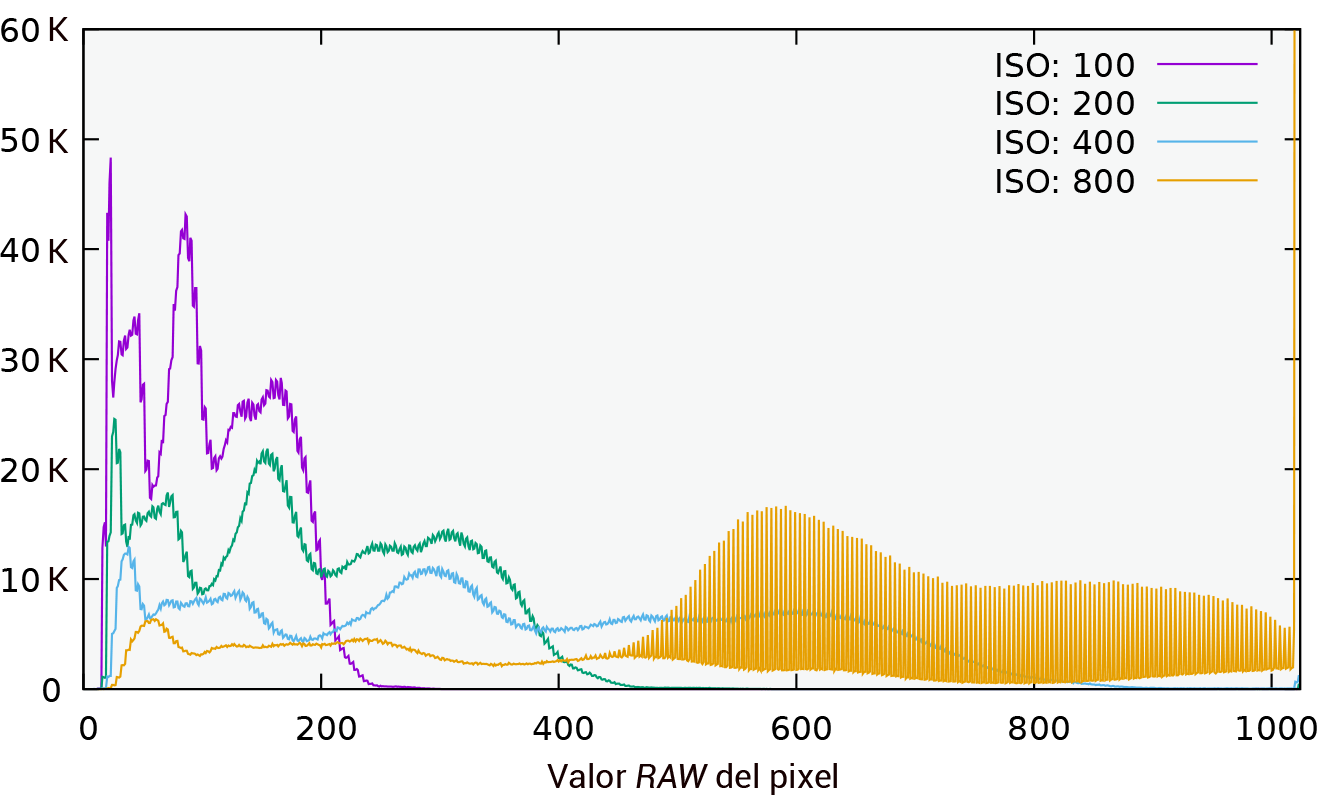
\includegraphics[width=0.9\textwidth]{figures/ISO.png}
        \label{fig:ISO}
        \caption{dependencia con el ISO}
      \end{subfigure}
      \begin{subfigure}{.47\textwidth}
        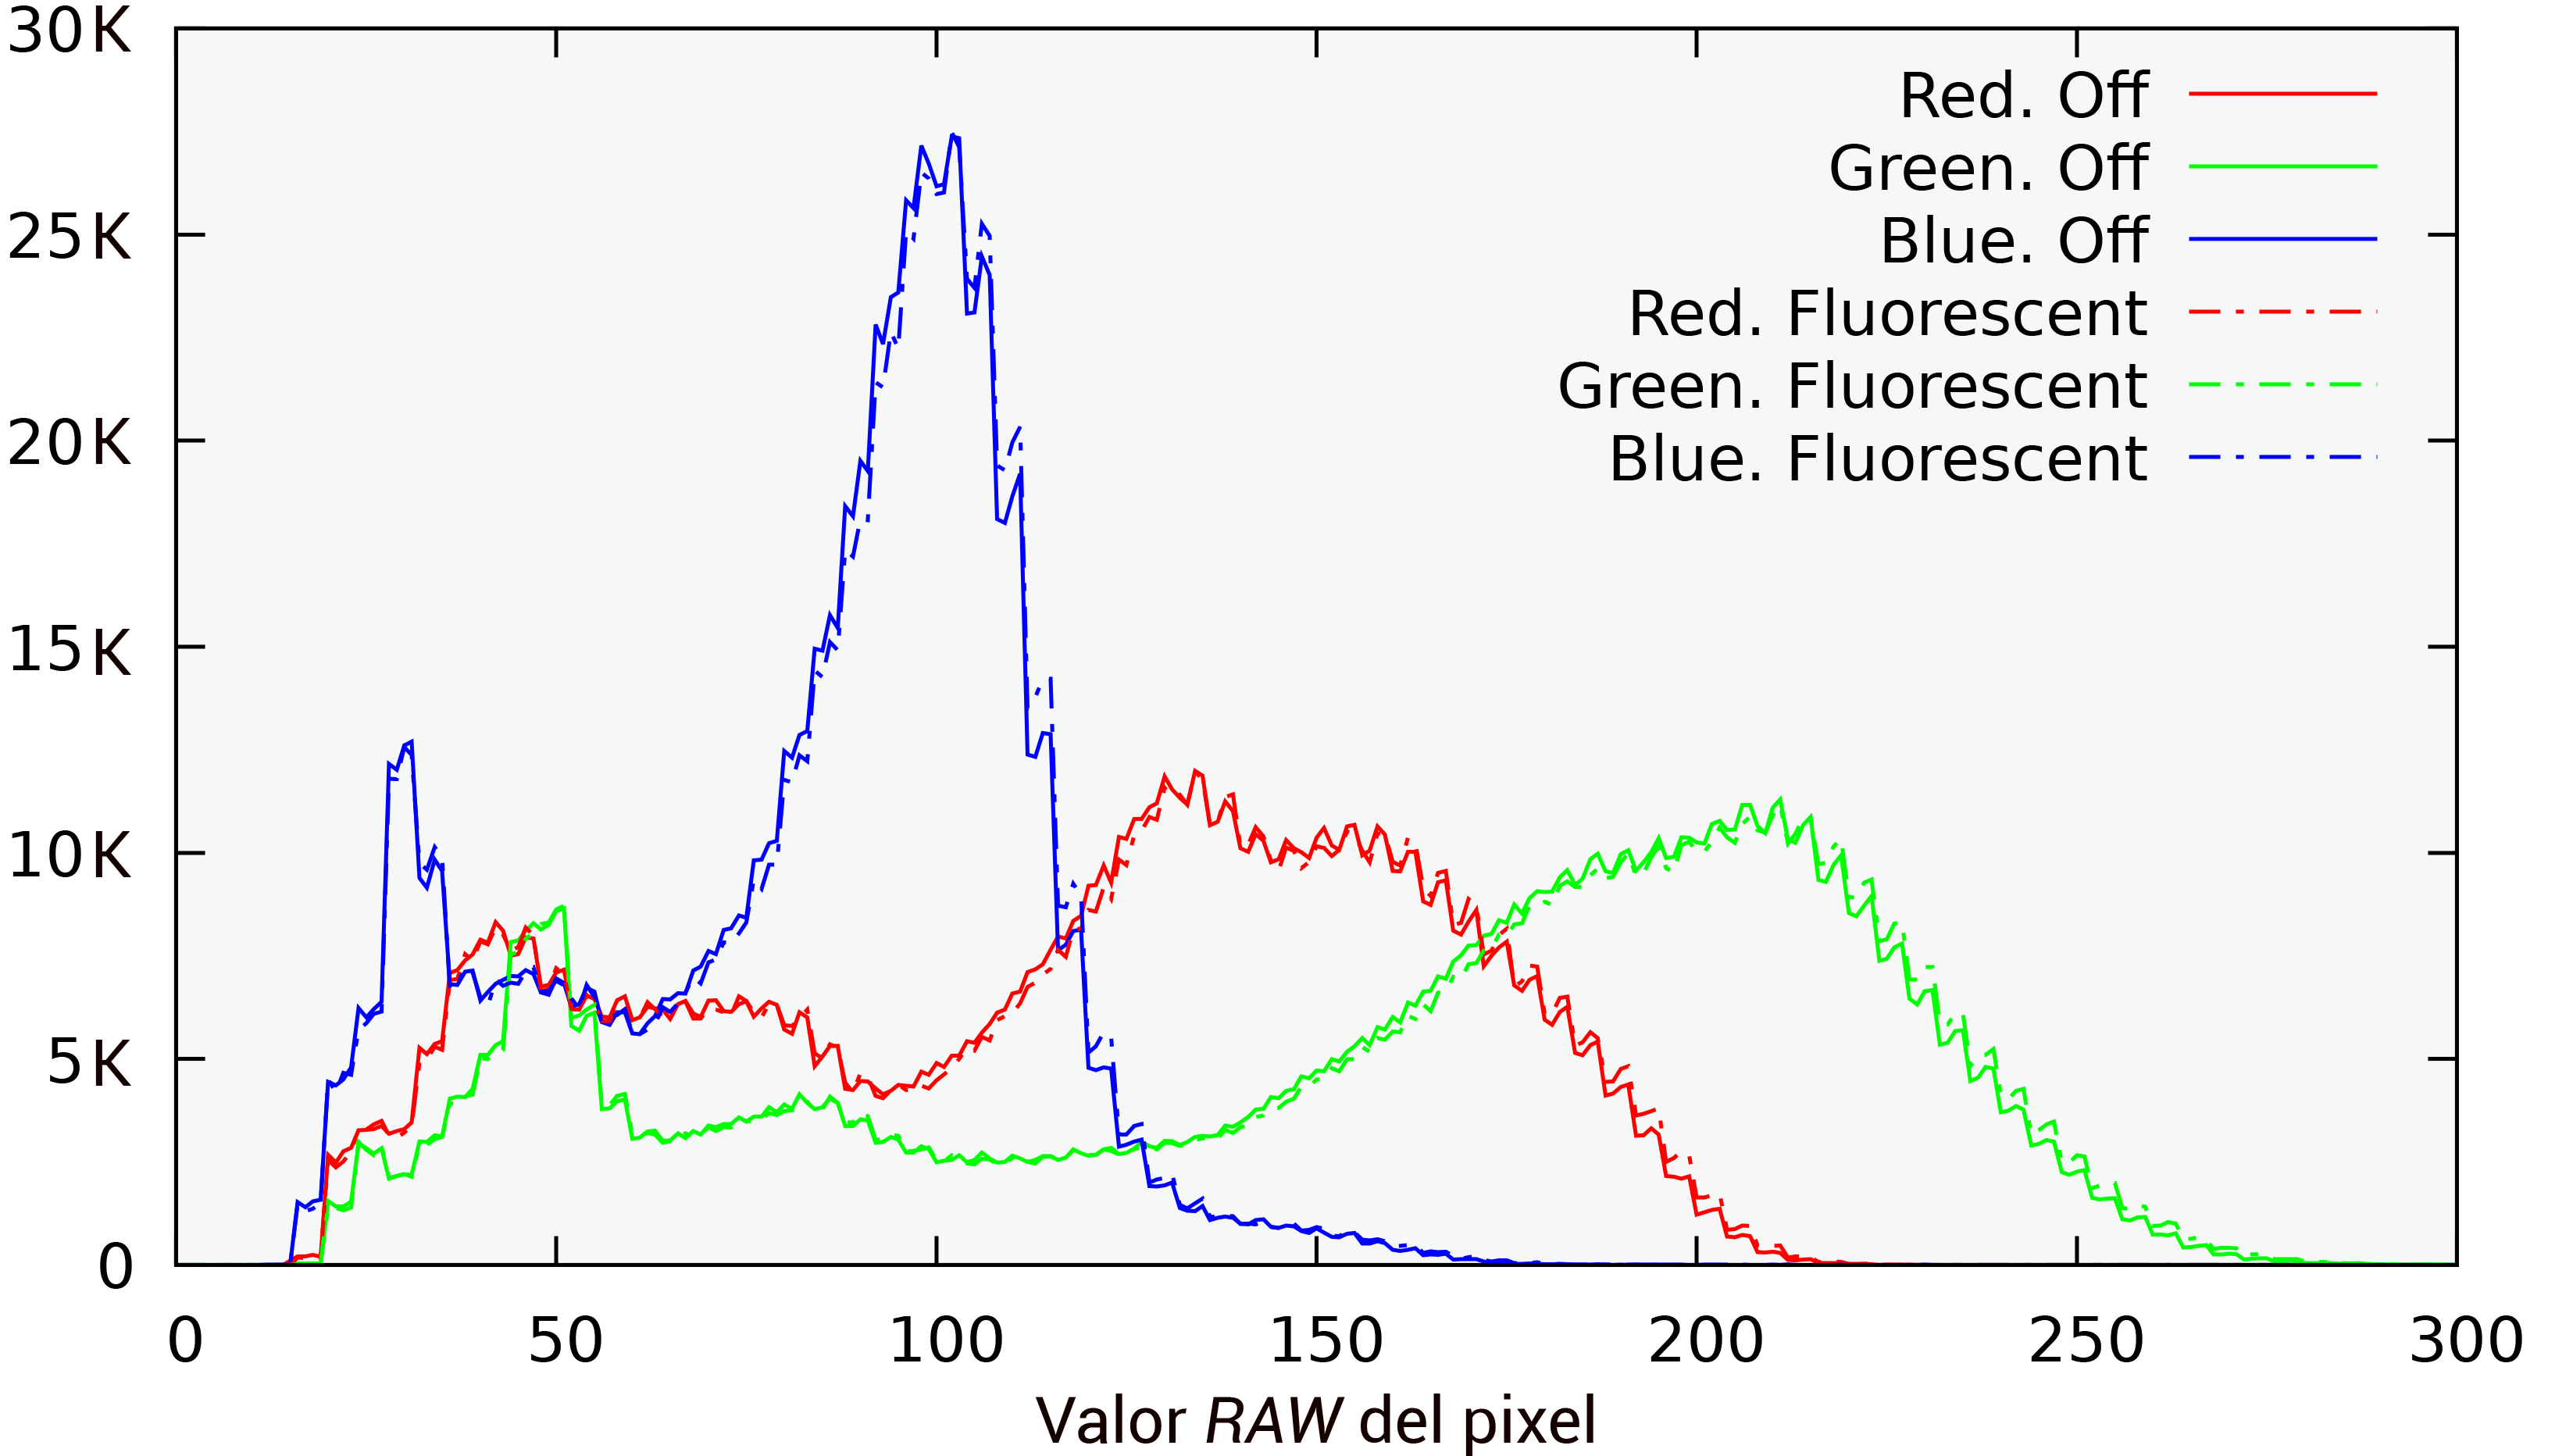
\includegraphics[width=0.9\textwidth]{figures/WB_component_transparent.png}
        \label{fig:WB}
        \caption{dependencia con el balance de blancos}
      \end{subfigure}
      \caption{Histogramas de los valores de los píxeles}
      \label{fig:histo_picamera}
    \end{figure}

    %TODO: Completar

\end{document}

    



